\documentclass[12pt, letterpaper]{article}
\usepackage{graphicx}
\usepackage[margin=1in]{geometry}
\usepackage{amsmath, amssymb, amsthm, mathrsfs}
\usepackage{fancyhdr}
\usepackage{tikz}
\usepackage{enumerate}
\usepackage{cancel}
\usetikzlibrary{positioning}
\usepackage[utf8]{inputenc}
\usepackage{xcolor}
\usepackage{framed}
\title{HW 1.3}
\author{Your Name}
\date{\today}
\pagestyle{fancy}
\renewcommand{\headrulewidth}{0pt}
\renewcommand{\footrulewidth}{0pt}
\fancyhf{}
\rhead{
    Zack Abdirashid\\
    2/4/26 \\
    MATH 405
}
\rfoot{Page \thepage}
\begin{document}
\paragraph{\underline{1.2} \\ \\} 
\textbf{4.} If directions are ignored, are the two graphs in Figure $1.11$ isomorphic?
\begin{center}
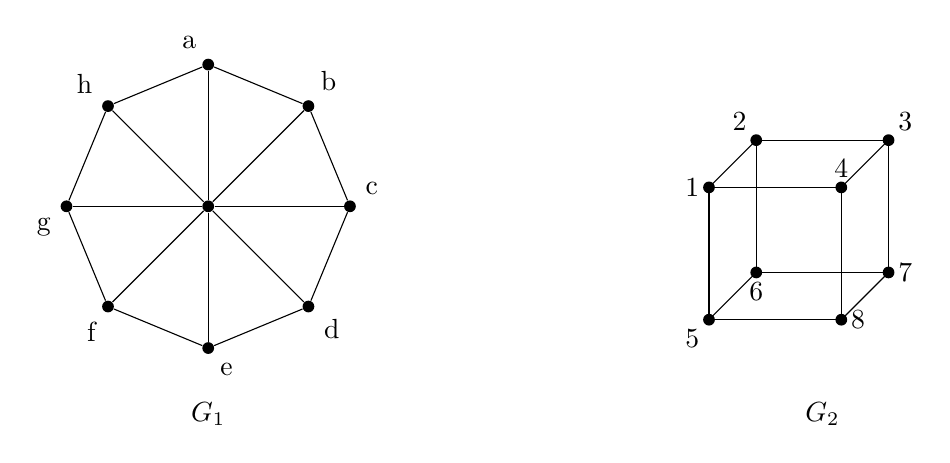
\begin{tikzpicture}[scale=1.2]
    % Left graph - Octagon with center
    \begin{scope}[xshift=-3cm]
        % Draw the octagon vertices
        %\foreach \i/\label in {0/a, 1/b, 2/c, 3/d, 4/e, 5/f, 6/g, 7/h} {
         \foreach \i/\label in {2/a, 1/b, 0/c, 7/d, 6/e, 5/f, 4/g, 3/h} {
            \node[circle, fill=black, inner sep=1.5pt, label={\i*45+22.5}:\label] (v\i) at (\i*45:1.5) {};
        }
        
        % Draw octagon edges
        \foreach \i in {0,1,2,3,4,5,6,7} {
            \pgfmathtruncatemacro{\next}{mod(\i+1,8)}
            \draw (v\i) -- (v\next);
        }
        
        % Draw center point
        \node[circle, fill=black, inner sep=1.5pt] (center) at (0,0) {};
        
        % Draw spokes from center to vertices
        \foreach \i in {0,1,2,3,4,5,6,7} {
            \draw (center) -- (v\i);
        }
        
        % Label
        \node at (0,-2.2) {$G_1$};
    \end{scope}
    
    % Right graph - Cube
    \begin{scope}[xshift=3.5cm]
        % Back face vertices
        \coordinate (v1) at (-0.7, 0.7);
        \coordinate (v2) at (0.7, 0.7);
        \coordinate (v3) at (0.7, -0.7);
        \coordinate (v4) at (-0.7, -0.7);
        
        % Front face vertices
        \coordinate (v5) at (-1.2, 0.2);
        \coordinate (v6) at (0.2, 0.2);
        \coordinate (v7) at (0.2, -1.2);
        \coordinate (v8) at (-1.2, -1.2);
        
        % Draw back face
        \draw (v1) -- (v2) -- (v3) -- (v4) -- cycle;
        
        % Draw front face
        \draw (v5) -- (v6) -- (v7) -- (v8) -- cycle;
        
        % Draw connecting edges
        \draw (v1) -- (v5);
        \draw (v2) -- (v6);
        \draw (v3) -- (v7);
        \draw (v4) -- (v8);
        
        % Draw vertices
        \foreach \i in {1,2,3,4,5,6,7,8} {
            \node[circle, fill=black, inner sep=1.5pt] at (v\i) {};
        }
        
        % Labels
        \node at (v1) [above left] {2};
        \node at (v2) [above right] {3};
        \node at (v3) [right] {7};
        \node at (v4) [below] {6};
        \node at (v5) [left] {1};
        \node at (v6) [above] {4};
        \node at (v7) [right] {8};
        \node at (v8) [below left] {5};
        
        % Label
        \node at (0,-2.2) {$G_2$};
    \end{scope}
\end{tikzpicture}
\end{center}
\begin{center}
    Both $G_1$ and $G_2$ have $8$ vertices each of degree $3$
\end{center}
\textbf{\underline{Bipartite Check}} \\ \\
\indent \ $G_1$: \ Start from vertex $a$ and consider the following circuit $C$\\
\begin{center}
     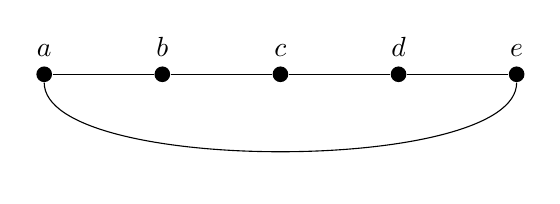
\begin{tikzpicture}
    % Draw vertices with proper styling
    \node[circle, fill=black, inner sep=2pt, label=above:$a$] (a) at (0,0) {};
    \node[circle, fill=black, inner sep=2pt, label=above:$b$] (b) at (1.5,0) {};
    \node[circle, fill=black, inner sep=2pt, label=above:$c$] (c) at (3,0) {};
    \node[circle, fill=black, inner sep=2pt, label=above:$d$] (d) at (4.5,0) {};
    \node[circle, fill=black, inner sep=2pt, label=above:$e$] (e) at (6,0) {};
    
    % Draw edges - straight lines along the top
    \draw (a) -- (b) -- (c) -- (d) -- (e);
    
    % Draw curved edge from f back to a
    \draw (e) to[out=-90, in=-90, looseness=0.5] (a);
\end{tikzpicture} \\
    \Rightarrow \text{$C$ is of odd length $\therefore$ $G_1$ is not bipartite.}
\end{center}
\indent \ $G_2$: Start from vertex $1$. \\
\begin{center}
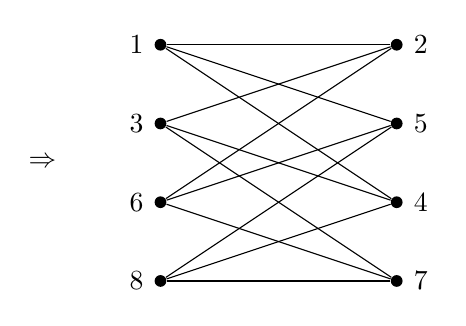
\begin{tikzpicture}[every node/.style={circle,fill,minimum size=1px,inner sep=1.5pt}]
    \node[fill=none, inner sep=0pt] at (-1.5,1.5) {$\Rightarrow$};
    \node[label=180:$1$] (1) at (0,3) {};
    \node[label=180:$3$] (3) at (0,2) {};
    \node[label=180:$6$] (6) at (0,1) {};
    \node[label=180:$8$] (8) at (0,0) {};
    
    \node[label=0:$2$] (2) at (3,3) {};
    \node[label=0:$5$] (5) at (3,2) {};
    \node[label=0:$4$] (4) at (3,1) {};
    \node[label=0:$7$] (7) at (3,0) {};
    
    \draw (1) -- (2);
    \draw (1) -- (5);
    \draw (1) -- (4);
    
    \draw (2) -- (3);
    \draw (2) -- (6);
    \draw (3) -- (4);
    \draw (3) -- (7);
    \draw (4) -- (8);
    \draw (5) -- (6);
    \draw(5) -- (8);
    \draw(6) -- (7);
    \draw(7) -- (8);
\end{tikzpicture} \\ \\
\Rightarrow \ $G_2$ is bipartite \therefore \boxed{\text{$G_1 \nsim G_2$}}
\end{center}
\end{document}